
\documentclass{standalone}
\usepackage{xcolor}
\usepackage{pgfplots}
\pgfplotsset{compat=1.18}

\begin{document}

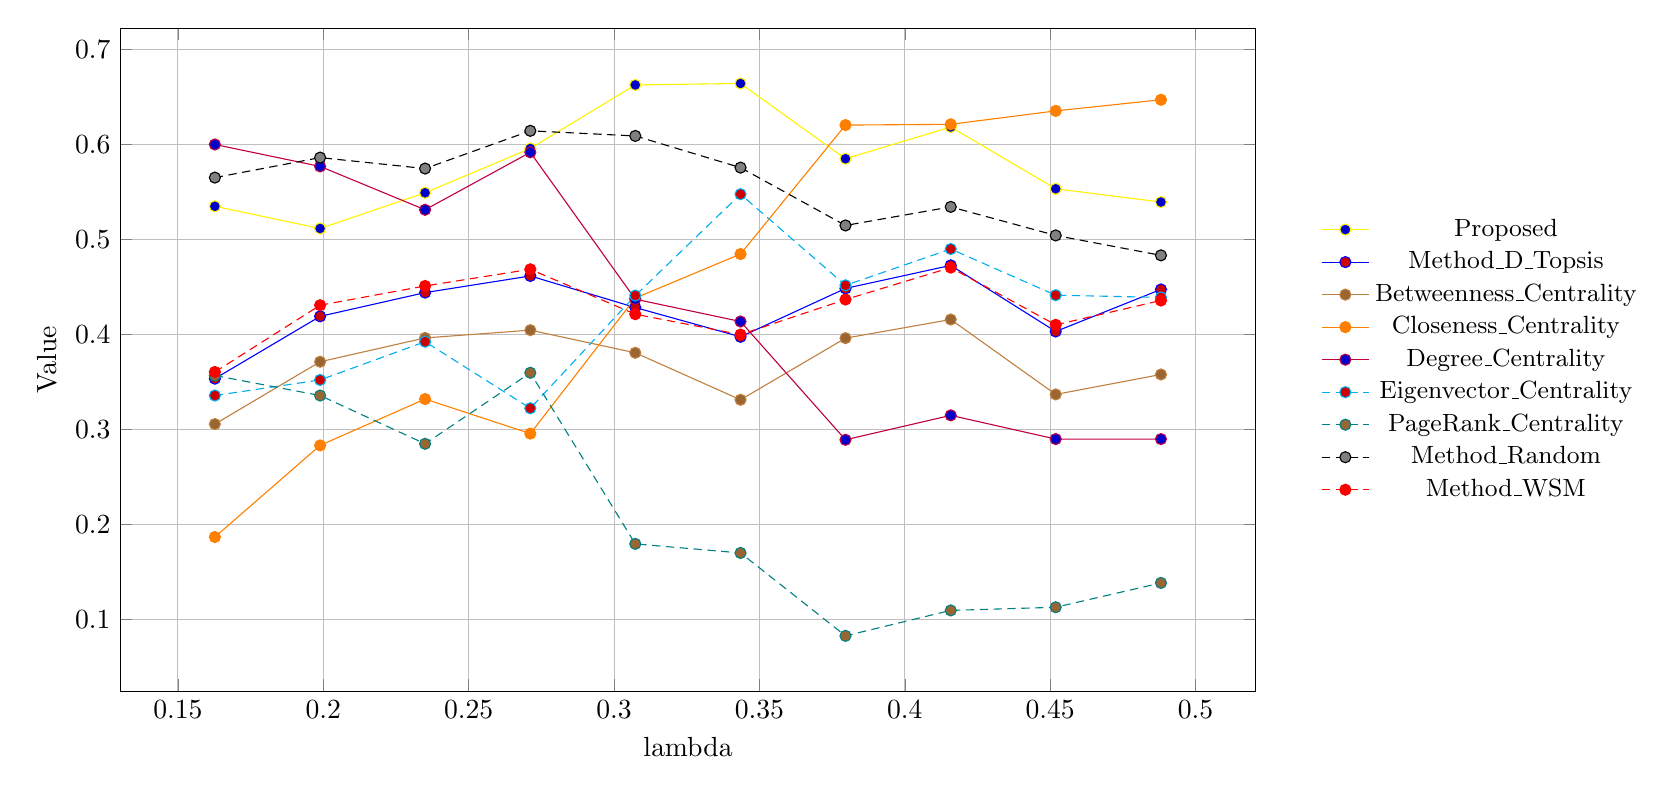
\begin{tikzpicture}
\begin{axis}[
    width=16cm,
    height=10cm,
    xlabel={lambda},
    ylabel={Value},
    grid=major,
    legend style={
        at={(1.05,0.5)},
        anchor=west,
        font=\small,
        draw=none,
        cells={align=left},
    },
]
% Proposed
\addplot+[color=yellow, mark=*] coordinates {
(0.1627,0.5347388488484202) (0.1989,0.5113878074139914) (0.235,0.5489525403396146) (0.2712,0.5955727136168644) (0.3073,0.6623985862210916) (0.3435,0.663953488372093) (0.3796,0.5847417195816498) (0.4158,0.618161070796836) (0.4519,0.5531668568918628) (0.4881,0.5392214739450091) };
\addlegendentry{Proposed}

% Method\_D\_Topsis
\addplot+[color=blue, mark=*] coordinates {
(0.1627,0.3534235989508681) (0.1989,0.418959100743082) (0.235,0.4439252336448598) (0.2712,0.4614485981308411) (0.3073,0.4282383312105244) (0.3435,0.3974369771885533) (0.3796,0.4483363285831411) (0.4158,0.4725790848508512) (0.4519,0.4030302470138344) (0.4881,0.4472936845471457) };
\addlegendentry{Method\_D\_Topsis}

% Betweenness\_Centrality
\addplot+[color=brown, mark=*] coordinates {
(0.1627,0.3056208184250196) (0.1989,0.3711946338725334) (0.235,0.396259565048312) (0.2712,0.4044419159490146) (0.3073,0.3806193811305015) (0.3435,0.3311967428428912) (0.3796,0.3960283076226927) (0.4158,0.4156457045474188) (0.4519,0.336831895811482) (0.4881,0.3578110450315743) };
\addlegendentry{Betweenness\_Centrality}

% Closeness\_Centrality
\addplot+[color=orange, mark=*] coordinates {
(0.1627,0.1868395289147264) (0.1989,0.2831970218141451) (0.235,0.3319676071725041) (0.2712,0.2956036643373535) (0.3073,0.4382017555797977) (0.3435,0.4845038923419187) (0.3796,0.6201709453770339) (0.4158,0.6209810974793925) (0.4519,0.635103357615928) (0.4881,0.6467995520471606) };
\addlegendentry{Closeness\_Centrality}

% Degree\_Centrality
\addplot+[color=purple, mark=*] coordinates {
(0.1627,0.5997624377616961) (0.1989,0.5766946516939386) (0.235,0.5310677535293734) (0.2712,0.5915144897034486) (0.3073,0.4370090065753058) (0.3435,0.4135268470619166) (0.3796,0.2891119843023048) (0.4158,0.3148189882894472) (0.4519,0.2898746529748299) (0.4881,0.2898746529748299) };
\addlegendentry{Degree\_Centrality}

% Eigenvector\_Centrality
\addplot+[color=cyan, mark=*] coordinates {
(0.1627,0.335673432984897) (0.1989,0.3520477467890383) (0.235,0.3922942875102485) (0.2712,0.3222417361691327) (0.3073,0.4408164014681704) (0.3435,0.5474673470186762) (0.3796,0.4515752625437573) (0.4158,0.4897960016313004) (0.4519,0.4412119060187319) (0.4881,0.4388836110001634) };
\addlegendentry{Eigenvector\_Centrality}

% PageRank\_Centrality
\addplot+[color=teal, mark=*] coordinates {
(0.1627,0.3567261221616501) (0.1989,0.335673432984897) (0.235,0.2848803754538709) (0.2712,0.3596030968843945) (0.3073,0.1795918672648101) (0.3435,0.1700643248185674) (0.3796,0.0828471411901983) (0.4158,0.10962100988891) (0.4519,0.1129223084005725) (0.4881,0.1385335536048261) };
\addlegendentry{PageRank\_Centrality}

% Method\_Random
\addplot+[color=black, mark=*] coordinates {
(0.1627,0.5649138262428753) (0.1989,0.5859665154196285) (0.235,0.5744309209971495) (0.2712,0.6141273667571152) (0.3073,0.6087464591703305) (0.3435,0.5754231264409064) (0.3796,0.514585764294049) (0.4158,0.5341108779693705) (0.4519,0.5040758715200816) (0.4881,0.483121216352965) };
\addlegendentry{Method\_Random}

% Method\_WSM
\addplot+[color=red, mark=*] coordinates {
(0.1627,0.3604452598571768) (0.1989,0.4306618689202631) (0.235,0.4509345794392523) (0.2712,0.4684579439252336) (0.3073,0.4212371595831045) (0.3435,0.3997679858524158) (0.3796,0.4366609033596219) (0.4158,0.4702453609750446) (0.4519,0.4100192108348836) (0.4881,0.4356454115120638) };
\addlegendentry{Method\_WSM}


\end{axis}
\end{tikzpicture}

\end{document}
